% Hier können die einzelnen Kapitel inkludiert werden. Sie müssen in den 
% entsprechenden .TEX-Dateien vorliegen. Die Dateinamen können natürlich 
% angepasst werden.

\chapter{Einleitung}
\label{cha:Einleitung}

\section{Motivation}
In der heutigen Zeit treten eingebettete Systeme (engl. embedded systems) immer st"arker in den Vordergrund. Gerade in den Bereichen der Industrie, Telekommunikation oder Multimedia w"achst der Bedarf an L"osungen die durch Zuverl"assigkeit, Energiesparsamkeit und kompakter Bauform bestechen.\\
Obwohl eingebettete Systeme meist f"ur den Anwender unsichtbar ihren Dienst verrichten, sind sie doch inzwischen allgegenw"rtig. Im Bereich der Telekomunikation und Unterhaltungselektronik kommt ein solches System im prinzip nicht mehr ohne ein Display aus. Die Moeglichkeit zur Anzeige multimedialer Daten wird zur Kaufentscheidung. Auch hier gilt die Maxime: besser, schneller, groesser.\\
Im Sektor der eingebetten Systeme mit Betriebssystem spielt Linux neben diversen anderen Systemen wie beispielsweise RTOS, OSEK, QNX oder auch Windows eine sehr grosse Rolle. In Verbindung zeigen eingebettete Linuxsysteme mit Displays ein grosses Potential. Mit der beliebten ARM-Architektur lassen sich so kostenguenstige, leisttungsstarke Systeme aufbauen, die die gestellten Aufgaben gut erfuellen kann.


\section{Ziel der Arbeit}
Das Ziel dieser Arbeit ist zu zeigen, dass die Verwendung von Displays mit eingebetten Linux Systemen  je nach Anforderung einfach oder ueber Umwege realisierbar ist. 


\section{Aufbau der Arbeit}
Im ersten Teil der Arbeit werden theoretische Grundlagen gebildet, die fuer das Verstaendnis notig sind. Hier werden Standards wie z.B. HDMI bzw. DVI, LVDS und RGB behandelt. Es wird ein Ueberblick ueber ausgewaehlte embedded Linux Boards gegeben und diese Klassifiziert mit welchen Displayschnittstellen diese ausgestattet sind bzw. ausgestattet werden koennen.
Der Zweite Teil behandelt das embedded Linux Board 'Gnublin', welches von Haus aus keine Displayschnittstelle vorgesehen hat. Hier werden zwei Varianten zur Ansteuerung von Displays erarbeitet. Die Ansteuerung wird hierbei vom Prozessor erledigt, da das 'Gnublin' keine dedizierten Grafikcontroller besitzt.
Im dritten Teil wird fuer leistungsstaerkere embedded Linux-Systeme mit HDMI-Schnittstelle eine Hardware entwickelt, RGB- oder LVDS-Panels anzuschliessen. Um die Displys ueber die entwickelte Hardware anzusteuern, wird der dedizierte Grafikcontroller der Boards verwendet.

\section{Typographische Konventionen}

\chapter{Theoretische Grundlagen}
\label{cha:Grundlagen}

\section{Embedded Linux Boards}

\section{Video-Schnittstellen}
\subsection{DVI}
\subsection{HDMI}
\subsection{VGA}
\subsection{8080-Interface}
\subsection{TV-OUT}
\chapter{Teil A}
\label{cha:TeilA}
Im Folgenden wird die Ansteuerung von TFT-Displays über den 8080-Bus auf Basis des \code{Gnublin Linuxboards} realisiert. Hierzu werden verschieden große LCD-Displays mit unterschiedlichen Controllern unter Verwendung des 8080-Interface untersucht. 

\section{Untersuchte Displays mit 8080-Interface}
Dieser Abschnitt beschreibt die drei untersuchten Displays. Der Fokus bei der Beschaffung lag vor allem darauf, dass die Pinbelegung der jeweiligen Displays übereinstimmt. So ist die Entwicklung von nur einer Adapterplatine zwischen \code{Gnublin Extended} und Display nötig. Alle verwendeten Displays werden im 16 Bit Farbmodus betrieben. Dieser entspricht einer resultierenden Farbtiefe von 65.535 Farben\newline % \footnote{2^16 = 65.536}.
Alle verwendeten Displays arbeiten dahingehend gleich, dass sie Kommandos und Daten auf dem Datenbus anlegen, diese jedoch durch eine gesonderte Leitung unterschieden werden. Soll dem Display also etwas mitgeteilt werden, so muss zuerst ein entsprechendes Kommando und im Anschluss die Nutzdaten gesendet werden. Um Pixeldaten an das Display zu senden, hat sich die Vorgehensweise etabliert, eine durch vier Eckpunkte definierte Region im RAM des Displays zu reservieren (siehe \refa{fig:ram_window}). Werden im Anschluss Pixeldaten gesendet, inkrementiert der Controller die Adresse und springt bei einem Zeilenumbruch automatisch an die richtige Stelle im RAM. Der verfügbare Speicher im Controller beschränkt dabei die maximale Auflösung der ansteuerbaren TFT-Panel. Trotz der Tatsache, dass sich die Displays auf elektrischer Seite nicht unterscheiden, müssen diese allerdings softwareseitig, aufgrund unterschiedlicher Displaycontroller, speziell behandelt werden.
\begin{figure}[h]
	\centering
\fbox{	\includegraphics[width=0.5\textwidth]{TeilA/ram_window.png}}
	\caption{Fensterreservierung im Display-RAM}
	\label{fig:ram_window}
\end{figure}
\subsection{4.3 / 5 Zoll mit SSD1963}
Die Wahl des Controllers \code{SSD1963} von Solomon Systech liegt nahe, da dieser bereits mit einem 4.3 Zoll  Panel in einer vorausgehenden Arbeit (siehe \cite{Schlegel2013a}) verwendet wird. Dort ist das Display mittels GPIO-Pins am Raspberry Pi angeschlossen. Die Software bezüglich der reinen Displayansteuerung ist somit bereits vorhanden. Aufgrund eines Problems, das in Abschnitt \ref{teila_knownbugs} näher beschrieben ist, ist ein weiteres Display mit 5 Zoll Panel aber demselben Controller untersucht. 
\refa{fig:8080_pinout} zeigt das Pinout der verwendeten Displays (Quelle: \cite{Coldtears2014}).
\begin{figure}[h]
	\centering
\fbox{	\includegraphics[width=0.5\textwidth]{TeilA/display_pinout.png}}
	\caption{8080-Display Pinout}
	\label{fig:8080_pinout}
\end{figure}
Die Displays haben bei 4.3 Zoll eine Auflösung von 480x272 beziehungsweise bei 5 Zoll 800x480 Pixel. Neben den für die Initialisierung nötigen Kommandos besitzt der Controller folgende wichtige Kommandos (siehe \reft{tab:Kommandos_SSD1963}, Quelle: \cite{SSD2008}). Die Initialisierungsbefehle sind nicht erläutert, da diese aus dem Datenblatt entnehmbar sind.
\begin{table}[h]
\begin{tabular}{|p{4cm}|p{1cm}|p{8cm}|}\hline
\rowcolor{TableBackgroundColor} 
   \textbf{Kommando} & \textbf{Hex-Code} & \textbf{Kommentar}\\ \hline
   Set Column Address & 0x2A & Eckpunkte des RAM-Fensters in X-Richtung \\ \hline
   Set Page Address & 0x2B & Eckpunkte des RAM-Fensters in Y-Richtung \\ \hline
   Write Memory Start & 0x2C & Alle Folgenden Pixeldaten werden im RAM-Fenster platziert \\ \hline
\end{tabular}
\caption{Relevante Kommandos des SSD1963}
\label{tab:Kommandos_SSD1963}
\end{table}
\subsection{3.2 Zoll mit SSD1289}
Das 3.2 Zoll Display von Sainsmart wird mit einen \code{SSD1289} von Solomon Systech betrieben. Dieses Display hat eine Auflösung von 320x240 Farbpunkten. Das Pinout ist dasselbe, das in \refa{fig:8080_pinout} zu sehen ist. Analog zu den Kommandos des \code{SSD1963} in \reft{tab:Kommandos_SSD1963} besitzt der \code{SSD1289} ähnlich Befehle. Diese sind in  \reft{tab:Kommandos_SSD1289} erläutert (siehe \cite{SSD2007}). Die zur Initialisierung notwendigen Kommandos sind hier nicht näher beschrieben, da diese wie zuvor aus dem Datenblatt entnehmbar sind.
\begin{table}[h]
\begin{tabular}{|p{4cm}|p{1cm}|p{8cm}|}\hline
\rowcolor{TableBackgroundColor}
   \textbf{Kommando} & \textbf{Hex-Code} & \textbf{Kommentar}\\ \hline
   Horizontal RAM address position & 0x44 & Eckpunkte des RAM-Fensters in X-Richtung \\ \hline
   Vertical RAM address start position & 0x45 & Startpunkt des RAM-Fensters in Y-Richtung \\ \hline
   Horizontal RAM address stop position & 0x46 & Endpunkt des  RAM-Fensters in Y-Richtung \\ \hline
   Set GDDRAM X address counter & 0x4E & Zeiger im  RAM-Fenster in X-Richtung \\ \hline
   Set GDDRAM Y address counter & 0x4F & Zeiger im RAM-Fenster in Y-Richtung \\ \hline
   RAM Write  Register & 0x22 & Alle Folgenden Pixeldaten werden im RAM-Fenster platziert \\ \hline
\end{tabular}
\caption{Relevante Kommandos des SSD1289}
\label{tab:Kommandos_SSD1289}
\end{table}


\subsection{5 Zoll mit CPLD}
Als drittes Display mit 8080-Interface kommt eine 5 Zoll Display mit einer Auflösung von 800x480 Bildpunkten zum Einsatz. Anstelle eines universell einsetzbaren Controllers für variable Panels, verwendet dieses Display ein CPLD\footnote{CPLD: Complex Programmable Logic Device} mit zugeschnittenen Timings für das verwendete TFT-Displays. Der Vorteil eines solchen Displays ist, dass keine Initialisierungsroutine benötigt wird, um die Timings für das Panel einzustellen. Ein Reset setzt das Display betriebsbereit. Nachteilig ist dabei, dass nur TFT-Panels exakter Größe und mit exakten Timings verwendet werden können. Für diese Arbeit ist die Verwendung von anderen Panels belanglos. Auch hier ist das Pinout des Displays analog zu \refa{fig:8080_pinout}.\newline
Wichtige Kommandos zum Betrieb des Displays sind in \reft{tab:Kommandos_MD050SD} einsehbar (siehe \cite{ITEAD2013}). Dieses Display trägt die Bezeichnung MD050SD.

\begin{table}[h]
\begin{tabular}{|p{4cm}|p{1cm}|p{8cm}|}\hline
\rowcolor{TableBackgroundColor}
   \textbf{Kommando} & \textbf{Hex-Code} & \textbf{Kommentar}\\ \hline
   Beginning Row Address & 0x02 & Startpunkt des RAM-Fensters in X-Richtung \\ \hline
   Ending Row Address& 0x06 & Endpunkt des RAM-Fensters in X-Richtung \\ \hline
   Beginning Column Address & 0x03 & Startpunkt des RAM-Fensters in Y-Richtung \\ \hline
   Ending Column Address& 0x07 & Endpunkt des RAM-Fensters in Y-Richtung \\ \hline
   Writing Page Register & 0x05 & Alle Folgenden Pixeldaten werden im RAM-Fenster platziert \\ \hline
\end{tabular}
\caption{Relevante Kommandos des MD050SD}
\label{tab:Kommandos_MD050SD}
\end{table}

% \input{Inhalt/TeilA/8080GPIO}
\section{8080-Interface mittels SRAM-Interface}
\label{sec:TeilA_8080SRAM}
Wie bereits in \refc{cha:gnublin_extended} erwaehnt, besitzt der Prozessor des Gnublin bereits ein externes 8080-Interface, auf welches zugegriffen wird. Im Folgenden wird auf das Konzept, die Idee und die Realisierung auf Hardware- und Softwareseite eingegangen.
\newpage
\subsection{Konzept}
Im Gnublin stellt ein NXP LPC313x die zentrale Recheneinheit dar. Dieser besitzt ein sogenanntes EBI \footnote{EBI: External Bus Interface}, worüber externe Bausteine wie Speicher, Ethernetcontroller oder ähnliche Bausteine angesprochen werden können. 


\begin{figure}[htp]
%\begin{minipage}[t]{0.8\textwidth}
%\begin{figure}[h]
	\centering
	\includegraphics[width=1.0\textwidth]{TeilA/lpc_ebi.png}
	\caption{NXP LPC313x EBI, Quelle: \cite{NXP2010}}
	\label{fig:lpc_ebi}
\end{figure}
%\end{minipage}

In \refa{fig:lpc_ebi} ist ein Blockschaltbild des EBI zu sehen, bei welchem neben CGU \footnote{CGU: Clock Generation Unit, Takterzeugung} und SYSCREG\footnote{SYSCREG: System Control Register, Steuerregister}, MPMC\footnote{MPMC: Multiport Memory Controller} sowie das NAND Flash an den Eingängen des EBI angeschlossen sind. An den Ausgängen des EBI sind Adress- und Datenbus zum Anschluss an externe Bausteine herausgeführt. Damit verschiedenartigen Bausteine an denselben Adress- und Datenpins angeschlossen werden kann, ist eine Priorisierung notwendig. Die Höchste Priorität besitzt der MPMC, gefolgt vom NAND Flash. 
Die Grundidee ist, das Display über den MPMC anzuschließen, da er so konfiguriert werden kann, dass er sich 8080-konform verhält.


\subsection{MPMC - Multiport Memory Controller des NXP LPC313x}

Der MPMC stellt die Möglichkeit zur Verfügung Bausteine wie dynamisches und statisches RAM anzubinden. Die Refresh-Zyklen werden bei Verwendung von dynamischen RAMs automatisch vollzogen. Das SDRAM-Interface bietet von Haus aus die Möglichkeit Displays mit 8080-Interface zu betreiben. Dies schließt allerdings die Verwendung von dynamischen RAMs aus. Soll ein Betriebssystem wie Linux laufen, ist allerdings die Verwendung von dynamischem RAM unerlässlich. Im Folgenden wird die Schnittstelle für das statische RAM SRAM-Interface benannt. Es besteht die Möglichkeit das Interface des statischen RAM zu verwenden, um ein Display zu betreiben, da es sich so konfigurieren lässt, dass es sich wie ein 8080-Interface verhält. Damit sich die verschiedenen Slaves an Adress- und Datenbus nicht überschneiden, regelt das EBI den Zugriff auf die Busse über Chip-Select Leitungen. Am Gnublin ist eine dieser Chip-Select-Leitungen fuer das SRAM-Interface nach außen gelegt. Die restlichen Anschlüsse wie Write-Enable, Read-Enable sind ebenfalls herausgeführt \cite{NXP2010}.


\begin{figure}[tbph]
%\begin{figure}[h!]
	\centering
	\includegraphics[width=1.0\textwidth]{TeilA/lpc_mpmc.png}
	\caption{NXP LPC313x MPMC, Quelle: }
	\label{fig:lpc_mpmc}
\end{figure}
\newpage
Die Register des MPMC werden so konfiguriert, dass die Schnittstelle kompatibel zum Display und dessen Timings wird. Entsprechend dem verwendeten Chip-Select-Signal werden die Register MPMCStaticConfig0, MPMCStaticWaitWen0, MPMCStaticWaitOen0, MPMCStaticRd0, MPMCStaticPage0, MPMCStaticWr0 und MPMCStaticWaitTurn0 entsprechend \reft{tab:mpmc_config} konfiguriert. Die Basisadresse des MPMC ist 0x1700 8000.

\begin{table}[h]
\begin{tabular}{|p{4cm}|p{1cm}|p{1cm}|p{6.6cm}|}\hline
%\begin{tabular}{|c|c|c|c|}\hline
	\textbf{Register} 	& \textbf{Offset} 	& \textbf{Wert} & \textbf{Beschreibung} 							\\ \hline
	MPMCStaticConfig0 	& 0x200 		& 0x81 			& 16 Bit Modus, Aktiviert die Nutzung von EBI\_nWE 	\\ \hline
	MPMCStaticWaitWen0 	& 0x204 		& 13 			& 13 + 1 = 14 Wartezyklen ab Chi- Select bis Write-Enable 	\\ \hline
	MPMCStaticWaitOen0 	& 0x208 		& 0 			& 0 + 1 = 1 Wartezyklus ab Chip-Select bis Output-Enable  												\\ \hline
	MPMCStaticRd0 		& 0x20C 		& 0 			& 0 + 1 = 1 Wartezyklus ab Chip-Select bis Read-Enable					\\ \hline
	MPMCStaticPage0 	& 0x210 		& 0 			& 0 + 1 = 1 Wartezyklus für sequential Page Mode Access												\\ \hline
	MPMCStaticWr0 		& 0x214 		& 15 			& 15 + 2  = 17 Wartezyklen bis Write-Access	\\ \hline
	MPMCStaticWaitTurn0 & 0x218 		& 0 			& 0 + 1 = 1 Turnaround Cycles 								\\ \hline
\end{tabular}
\caption{MPMC Register}
\label{tab:mpmc_config}
\end{table}


\subsection{Hardwareverbindung zwischen SRAM-Interface und Display (Adapterplatine)}

\subsection{Software}
\subsubsection{Entwicklung eines Linux-Framebuffer-Treibers}
\paragraph{Anpassungen für Display mit SSD1289 Controller}
\paragraph{Anpassungen für Display mit SSD1963 Controller}
\paragraph{Anpassungen für Display mit CPLD Controller}
\subsubsection{Entwicklung eines User-Space-Treibers}
\paragraph{Anpassungen für Display mit SSD1289 Controller}
\paragraph{Anpassungen für Display mit SSD1963 Controller}
\paragraph{Anpassungen für Display mit CPLD Controller}
\subsubsection{Anpassung des APEX-Bootloaders zur Verwendung des Displays}
\subsubsection{Probleme bei der Entwicklung und Fehlersuche}
\paragraph{Probleme mit SSD1963}
\subparagraph{Rolle des User-Space-Treibers}
\subparagraph{Debuggen mit Logik-Analyzer}





% \section{Vor- und Nachteile}
\section{Known Bugs}
Im Laufe der Entwicklung gab es Erschwernisse, welche die Entwicklung verzögerten. 
Als Einschränkung bezüglich des MD050SD, stellt sich die begrenzte Geschwindigkeit von 50~MHz dar. Mit einer maximalen Busgeschwindigkeit von 90~MHz, könnte das Display wesentlich schneller betrieben werden, was die Framerate fast verdoppeln würde. Zusätzlich erscheinen auf dem Display zufällig Artefakte in Form von einzelnen Pixeln, was die Vermutung zulässt, dass die Leitungen von der Adapterplatine oder des MD050SD selbst anfällig für Störungen von außen sein können. \\ \\
Bezüglich dem SSD1289 stellte sich heraus, dass die Verwendung der angebotenen Kommandos aus \reft{tab:Kommandos_SSD1289} nicht für die Adressierung eines RAM-Fensters über mehrere Zeilen zuverlässig funktioniert. Unabhängig vom gesendeten Kommando treten hier zufällige Resets des Displaycontrollers auf, welche das Display nach kurzer Zeit komplett weiß erscheinen lässt. Als Lösung stellte sich die Reservierung einzelner Zeilen dar, die in der Summe das komplette RAM-Fenster abdecken. Nachteilig stellt sich hierbei der erhöhte Adressierungsaufwand dar, da jede Zeile erneut adressiert werden muss.\\ \\
Der Betrieb mit dem SSD1963 stellt sich problematischer dar, als anfangs angenommen. Die Ursache des Problems ist noch ungeklärt, was den Betrieb mit dem SSD1963 derzeit unmöglich macht.
Das Problem stellt sich so dar, dass sich trotz scheinbar korrektem Datenverkehr auf dem 8080-Bus der Displaycontroller nicht initialisieren lässt. Als erster Schritt steht immer die PLL\footnote{PLL: Phase Locked Loop, Phasenregelschleife zur Erzeugung von hohen Taktraten}. Mithilfe der PLL wird der erforderliche Displaytakt von z.~B. 90~MHz erzeugt und der Controller mit dieser Frequenz betrieben. Ein solche schneller Zugriff auf den SSD1963 ist erst nach der Initialisierung der PLL möglich. Bevor dies der Fall ist, kann mit maximal 5 M Words/s \footnote{5M~Word/s: $5*10^6$ Datenwörter pro Sekunde} geschriebenen bzw. gelesen werden (siehe \cite{SSD2008}, S. 72). Der Fehler stellt sich so dar, dass sich die PLL nicht initialisieren lässt. Um den Fehler zu finden, wurden diverse Überlegungen vorangestellt. Angedachte potentielle Fehlerquellen sind
\begin{itemize}
\item zu flache Flanken der Signale
\item 8080-Bus Protokoll nicht eingehalten
\item 8080-Bus Timing nicht im Rahmen der Spezifikationen
\item 8080-Bus Datenverkehr fehlerhaft
\item Leitungsführung auf dem Display selbst schlecht
\end{itemize}
Die Flanken der Signale haben sich nach Messungen mit dem Oszilloskop als nicht zu flach herausgestellt und können als Fehlerquelle ausgeschlossen werden. Die Einhaltung des 8080-Bus Protokolls, samt der Einhaltung der Timings wurden ebenfalls überprüft. Hierzu ist dasselbe Display mit einer funktionierenden Displayansteuerung über die GPIO-Pins aufgebaut worden und jedes Kommando der Initialisierung des SSD1963 mit dem Logic-Analyzer aufgenommen worden. Derselbe Displaytreiber, mit dem Unterschied der Ansteuerung über das SRAM-Interface, wurde ebenfalls aufgezeichnet und mit den Daten der vorhergehenden Messung verglichen. Diese Methode schließt einen Fehlerhaften Datenverkehr aus und lässt zusätzlich die Rahmenbedingungen für das 8080-Interface selbst und dessen Timing überprüfen. Für die Aufzeichnung, wurde der User-Space-Treiber dahingehend modifiziert, dass er vor dem Senden die Bestätigung des Anwenders abfragt. Die Abbildungen \ref{fig:ssd1963_gpio} und \ref{fig:ssd1963_sram} zeigen einen exemplarischen Datentransfer für die beiden Ansteuerungsmethoden. Zu erkennen ist, dass dasselbe Wort an den Datenpins D[7:0] anliegt, und die Steuersignale CS, WR, RD und A15 entsprechend innerhalb der markierten Zonen entsprechend dem 8080-Interface geschaltet werden. 

\begin{figure}[htp]
        \begin{center}
        \begin{subfigure}[htp]{1\textwidth}
			%\begin{figure}[h!]
			\centering
			\fbox{	\includegraphics[width=1\textwidth]{TeilA/print_34_dip.png}}
	\caption{SSD1963 mit GPIO}
			\label{fig:ssd1963_gpio}
		\end{subfigure}


        \begin{subfigure}[htp]{1\textwidth}
%\begin{figure}[h!]
	\centering
\fbox{	\includegraphics[width=1\textwidth]{TeilA/print_34_ext.png}}
	\caption{SSD1963 mit SRAM-Interface}
	\label{fig:ssd1963_sram}
\end{subfigure}

		\end{center}
\caption{SSD1963: Vergleich GPIO- und SRAM-Ansteuerung}
	\label{fig:ssd1963_gpio_sram}
\end{figure}
\newpage
Das geforderte Timing ist in \refa{fig:ssd1963_timing_constraints} zu sehen und beinhaltet die minimal notwendigen Zeiten zwischen den einzelnen Signalen.
\begin{figure}[htp]
%\begin{minipage}[t]{0.8\textwidth}
%\begin{figure}[h]
	\centering
\fbox{	\includegraphics[width=1.0\textwidth]{TeilA/ssd1963_writeCycleConstraings.png}}
	\caption{8080-Timingbedingung für SSD1963}
	\label{fig:ssd1963_timing_constraints}
\end{figure}
Diese Mindestzeiten wurden innerhalb der Oszilloskopbilder eingehalten und verifiziert, sodass ein Fehler mit dem Protokoll des 8080-Interface ausgeschlossen werden kann. Bezüglich der uninitialisierten PLL des Displays und der verringerten Schreibrate ist in \refa{fig:ssd1963_sram} eine Chip-Select-Laenge von 406~Nanosekunden erkennbar, was einer Schreibgeschwindigkeit von 2.46~MHz entspricht. Dies ist weit unter den geforderten 5~MHz im uninitialisierten Zustand. Ein zu schnelles Schreiben ist in diesem Fall ebenfalls ausgeschlossen. Nachdem verifiziert wurde, dass aus der Adapterplatine vom Gnublin Extended die richtigen Signale geliefert werden, bleibt als Ursache nur noch das Display selbst. Da die Leitungsführung des ursprünglich verwendeten 4.3" Displays nicht optimal ist, bei dem die 8080-Leitungen quer über die Platine geführt und im Anschluss von den RGB-Signalen im 90 Grad Winkel gekreuzt werden, wurde der Fehler im schlechten Platinendesign des Displays gesucht. Aufgrund dessen fand das 5" Display mit demselben Controller Verwendung, das eine optimierte Leitungsführung besitzt. Jedoch waren die aufgeführten Lösungsansätze nicht zielführend, weswegen das Display nicht mit dem Gnublin Extended unter Verwendung des SRAM-Interface einsetzbar ist.

\input{Inhalt/TeilA/TeilAZusammenfassung}


\chapter{Teil B}
\label{cha:TeilB}
Im Folgenden wird Teil B dieser Arbeit behandelt. Bei embedded-Linux Systemen mit höherer Leistung und vor allem einer dedizierten Grafikkarte, die es sogar ermöglicht 3D Beschleunigung in Hardware oder Full-HD Anzeige mittels HDMI-Monitoren, ist die Frage nicht, ob ein Display angeschlossen werden kann, sondern eher welches. Die HDMI-Schnittstelle bietet bereits die Möglichkeit eine Vielzahl von Anzeigegeräten anzuschließen. Befindet man sich allerdings im embedded Bereich, so sind die Anforderungen an die Kompaktheit der Baugröße, oft von sehr großer Bedeutung. Zu diesem Zweck wurde in Teil B dieser Arbeit eine Möglichkeit entwickelt, die den Anschluss von ausgewählten Displays mit einem Formfaktor von 7"' bei der Auflösung von 800x480 mit RGB- sowie LVDS-Schnittstelle auf kompaktem Raum mit dem HDMI-Anschluss des embedded-Boards verbinden lässt. Betrachtet man die entwickelte Hardware näher, wird klar, dass diese mit jeder erdenklichen HDMI-Quelle verwendbar ist und im weitesten Sinne einen kompakten HDMI-Monitor darstellt.
In den nachfolgenden Kapiteln werden die Konzeption sowie die entwickelte Hard- und Software behandelt. Im Anschluss folgt ein Kapitel, welches die bekannten Fehler im Projekt aufzeigt.\newpage
\section{Konzept}
\label{sec:TeilB_Konzept}
Um die Entwicklung zielführend zu gestalten ist neben der Bauteilrecherche eine grobe Hardwarearchitektur zu erstellen, welche sich zunehmend verfeinert. Die letztendliche Architektur wird als Ausgangspunkt für weitere Entwicklungen genommen. Treten Probleme während der Entwicklung auf, wie z. B. Bauteile sind nicht lieferbar, zu teuer oder die gewünschten Bauformen nicht verfügbar, sind Alternativen zu finden. Dabei steht im Mittelpunkt das Konzept bestenfalls nur minimal ändern zu müssen. Um solchen Probleme zu vermeiden, ist es sinnvoll ein vollständiges Konzept, sowie eine Bauteildatenbank inklusive Lieferdaten der Bauteile im Vorfeld zu erstellen. Das Projekt orientiert sich bezüglich der Konversion von HDMI nach RGB und LVDS an der Application Note SLLA325A von Texas Instruments (siehe \cite{TI2011}).
\begin{figure}[htp]
%\begin{minipage}[t]{0.8\textwidth}
%\begin{figure}[h]
	\centering
\fbox{	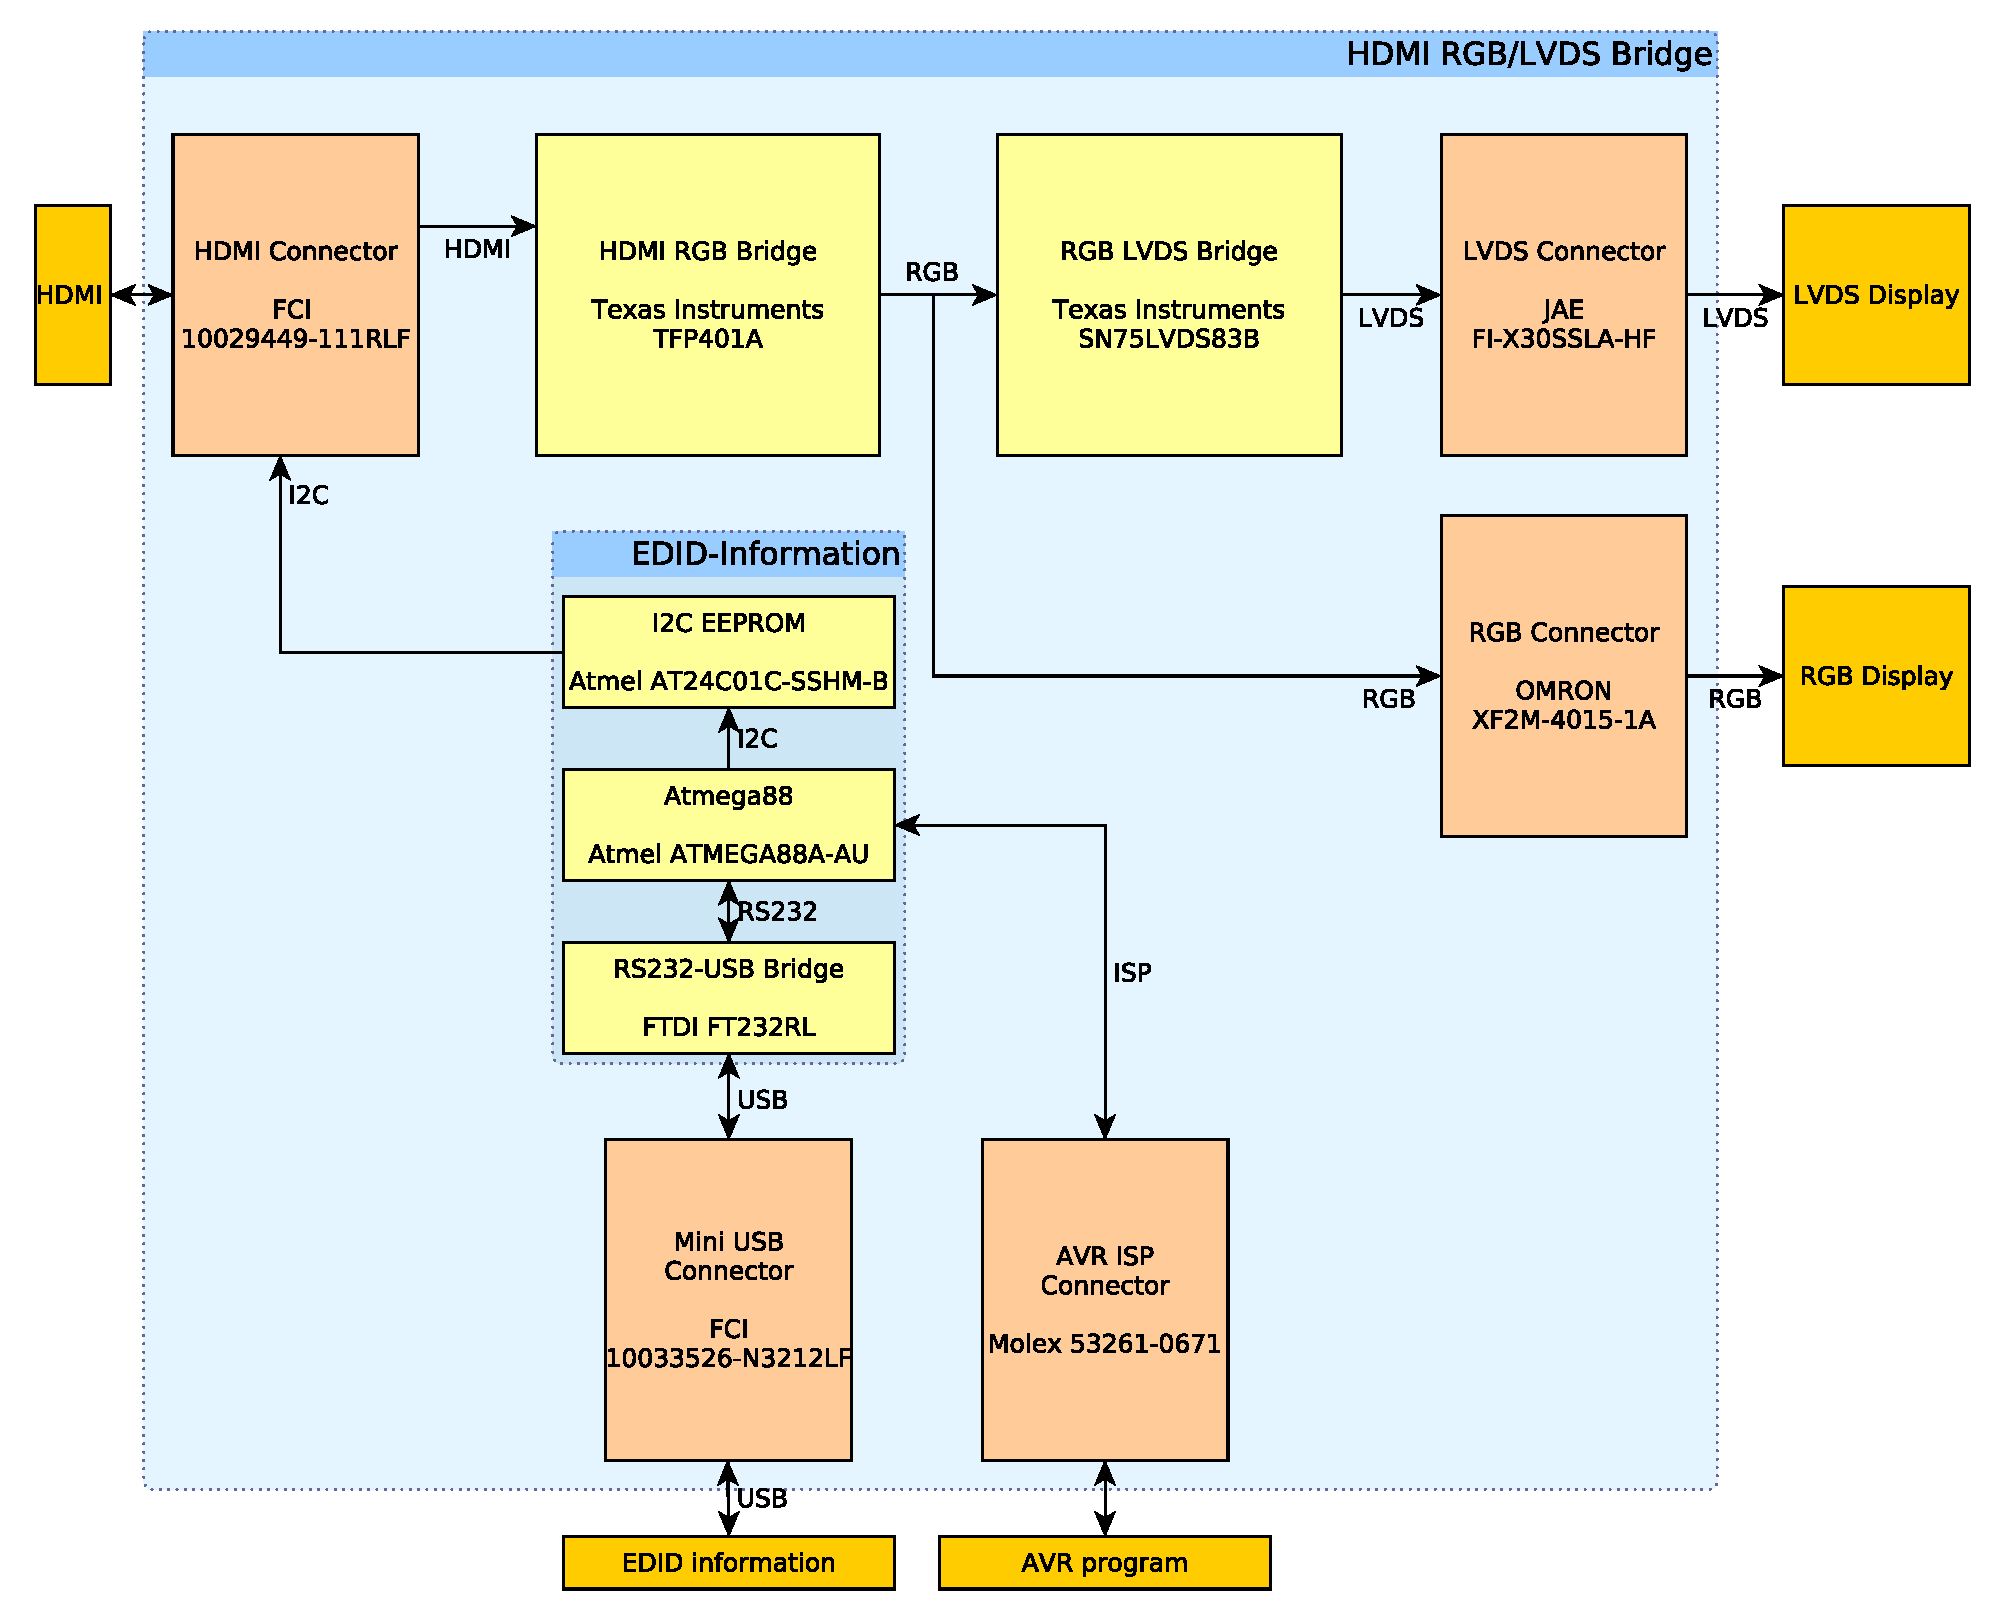
\includegraphics[width=1.0\textwidth]{TeilB/Architektur.pdf}}
	\caption{Hardware-Architektur}
	\label{fig:teilb_architektur}
\end{figure}

\refa{fig:teilb_architektur} zeigt die komplette Architektur des Projekts mit allen notwendigen Eckpunkten und Verbindungen. So sind Schnittstellen nach außen mit rot und die interne Logik mit gelb markiert. Als Signalquelle wird das HDMI-Signal eingespeist und in die \code{HDMI-RGB-Bridge} geleitet. Der Baustein \code{TFP401A} konvertiert die eingehenden HDMI-Signale zum RGB-Bus. Hier kann direkt über einen FPC-Stecker\footnote{FPC: Fine Pitch Connector} ein RGB-Display anschlossen werden. Die Leitungen werden zu einer RGB-LVDS-Bridge weitergeleitet. Diese wandelt die RGB-Signale in LVDS-Signale entsprechend der benötigten Beschaltung des verwendeten Displays um. Wird die Platine mit einer Quelle verbunden, so tauschen beide Informationen aus. Dabei ließt die Quelle Leistungsdaten bzgl. Auflösung, Timings, etc. aus einem EEPROM  im Anzeigegerät aus. Diese Daten werden als EDID-Daten\footnote{EDID: Extended Display Identification Data} bezeichnet (siehe \cite{edid2000}). Gespeichert werden die EDID-Daten üblicherweise in einem EEPROM\footnote{EEPROM: Electrically Eraseable Programmable Read-Only Memory}, auf welches mit dem $I^2C$-Bus zugegriffen wird. Um das EEPROM mit korrekten Inhalten beschreiben zu können, ist eine Baugruppe mit den Namen \code{EDID-Information} realisiert (siehe \refa{fig:teilb_architektur}). Der verwendete USB-Seriell-Konverter FT232RL kommuniziert mit einem 8-Bit Atmel ATMega88 Prozessor, welcher das $I^2C$-EEPROM direkt beschreiben kann. Um die korrekten EDID-Informationen in das EEPROM zu schreiben ist die zugehörige PC Software zu verwenden (siehe \refc{edid_pc}).\newpage

\section{Hardwareentwicklung}
\label{sec:TeilB_Hardware}

\subsection{Spannungsversorgung}
\subsection{HDMI-RGB-Bridge}
\subsection{RGB-LVDS-Bridge}
\subsection{EDID-Daten}


\section{Software}
\label{sec:TeilB_Software}

\subsection{EDID-Daten auf embedded Seite}
\subsubsection{Konzept}
\subsubsection{Low-Level-Treiber}
\paragraph{UART-Treiber}
\paragraph{I2C-Treiber}
\subsubsection{Programmablauf}

\subsection{EDID-Daten auf PC Seite}
\subsubsection{Konzept}
\subsubsection{GTK GUI mit Glade}
\subsubsection{Programmablauf}

\section{Known Bugs}
Im Rahmen der Entwicklung und mit Fortschreiten des Projekts sind, trotz Reviews der einzelnen Elementen des Projekts, Fehler bekannt geworden, die komplett oder teilweise gelöst oder umgangen wurden. Auf diese Fehler wird in den folgenden Abschnitten eingegangen.
\subsection{Hardware}
Bei der Hardwareentwicklung sind Schaltungstechnisch und bzgl. der erstellten Bauteilbibliothek Fehler aufgetreten. 
\subsubsection{HDMI-Stecker gekreuzt}
\textbf{Problem:} Durch einen Fehler beim Erstellen der HDMI-Buchse CON2 im Schaltplanprogramm \code{Eagle} wurde fälschlicherweise die Belegung des Steckers verwendet. Die Verwendung von normalen HDMI-Kabeln ist daher nicht möglich!\\
\textbf{Workaround:} Alle Signale müssen gekreuzt werden. Hierzu wird ein HDMI-Stecker an ein abgetrenntes Ende eines HDMI-Kabels verbunden. Dazu wird die Belegung entsprechend \refa{fig:hdmi_stecker_problem}\footnote{Quelle: \url{http://upload.wikimedia.org/wikipedia/commons/thumb/4/48/HDMI_Connector_Pinout.svg/1280px-HDMI_Connector_Pinout.svg.png}} gekreuzt.
\begin{figure}[htp]
	\center
	\fbox{\includegraphics[width=0.6\textwidth]{TeilB/hdmi_stecker_problem.png}}
    \caption{Known Bugs: HDMI-Stecker, }
    \label{fig:hdmi_stecker_problem}
\end{figure}\\
%    }}
\textbf{Lösung:} Um das Problem endgültig zu lösen, muss das Schaltplansymbol in \code{Eagle} sowie das Platinenlayout bzgl. der Beschaltung der HDMI-Buchse und der RGB-Bridge angepasst werden.
\subsubsection{LVDS-Steckerfootprint gespiegelt}
\textbf{Problem:} Das Schaltplansymbol des LVDS-Steckers CON6 muss gespiegelt werden. Das Anstecken des LVDS-Displays mit vorgesehener Belegung kann zur Zerstörung des Displays führen.\\
\textbf{Workaround:} Der LVDS-Stecker wird um 180 Grad gedreht auf die bereits dort vorgesehenen Pads angelötet.\\
\textbf{Lösung:} Das Schaltplansymbol muss in \code{Eagle} um 180 Grad gedreht werden.
\subsubsection{+5V-Kreis / Widerstand}
\textbf{Problem:} Der Widerstand \code{R13} wird verwendet um eventuell auftretende Spannungsunterschiede zwischen den +5\,V der USB- und HDMI-Versorgung auszugleichen (siehe \refa{fig:r13}). Dieser Widerstand ist mit 10\,k$\Omega$ zu groß gewählt.
\begin{figure}[htp]
	\center
	\fbox{\includegraphics[width=0.2\textwidth]{TeilB/r13.png}}
    \caption{Known Bugs: +5V-Kreis}
    \label{fig:r13}
\end{figure}\\
\textbf{Lösung:} Verkleinerung des Widerstands bzw. Entfernen und Brücken von \code{R13} mit 0\,$\Omega$.
\subsubsection{USB D+/D- vertauscht}
\textbf{Problem:} Die USB-Datensignale \code{USB_D+} und \code{USB_D-} sind vertauscht. Dies verhindert die Kommunikation zwischen PC und AVR (siehe \refa{fig:usb_vertauscht}).
\begin{figure}[htp]
	\center
	\fbox{\includegraphics[width=0.45\textwidth]{TeilB/usb_dp_dm.png}}
    \caption{Known Bugs: USB Signale vertauscht}
    \label{fig:usb_vertauscht}
\end{figure}\\
\textbf{Workaround:} Entfernen der 0\,$\Omega$ Widerstände \code{R22} und \code{R23} und kreuzen der Signale mit Fädeldraht.\\
\textbf{Lösung:} Um das Problem endgültig zu beheben, müssen die Signale \code{USB_D+} und \code{USB_D-} im Schaltplan am Baustein \code{FT232RL} getauscht und im Platinenlayout entsprechende Anpassungen gemacht werden.
\subsection{Software}
\textbf{Problem:} Unter bisher ungeklärten Umständen kann es vorkommen, dass die Prüfsumme des ausgelesenen EEPROMs und der im PC-Programm berechneten Software nicht übereinstimmt. \\
\textbf{Workaround:} Ein erneuter Programmiervorgang umgeht das Problem. Die Prüfsummen werden nun korrekt berechnet und verglichen.
\input{Inhalt/TeilB/TeilBZusammenfassung}
\chapter{Zusammenfassung}
\label{cha:Zusammenfassung}
Die Ziele der beiden Teile dieser Masterarbeit waren
\begin{itemize}
\item Optimierte Portierung des vorausgehenden Projekts zur Ansteuerung von TFT-Displays
\item Ausnutzung der vollen Grafikleistung von Linux-Boards mit Grafikhardware über die HDMI-Schnittstelle über eine selbst entwickelte Hardware zur Ansteuerung von Displays
\end{itemize}
Im Teil A dieser Arbeit ist auf die Low-Level Programmierung des verwendeten Prozessors \code{LPC 3131} eingegangen worden. Es wurde ein Verfahren entwickelt, Displays mit 8080-Interface an einem Speicherbus des Prozessors zu betreiben. Diese Methode findet in einem entwickelten Framebuffer-Treiber im Linux-Kernel, einem User-Space-Treiber sowie im Bootloader Verwendung.\newline

Hierbei ergaben sich Erschwernisse in der Entwicklung, die teilweise gelöst wurden aber noch Fragen bzgl. der Fehlerursachen offen lassen. 
So scheint die Verwendung der Grafikcontroller \code{SSD1963} im Vergleich zum \code{SSD1289} und dem Display \code{MD050SD} in der entwickelten Anwendung nicht nutzbar zu sein. Die Fehlerursache konnte trotz ausgedehnter Suche nach wie vor nicht ermittelt werden.\newline
Mit dem \code{MD050SD} lässt sich das Ziel der optimierten Ansteuerung unter Verwendung des Speicherinterface gut zeigen. Dabei wird gezeigt, dass es auch für leistungsschwache Systeme gute Möglichkeiten zur Anzeige gibt.\newline

Mit der vollen Ausnutzung der Grafikhardware ist das Linux-Board als Einheit zu sehen, welche über die HDMI-Schnittstelle verlassen wird. Die berechneten Video-Signale werden von einer Onboard-Grafikeinheit zur Verfügung gestellt, die mit der entwickelten Hardware aus Teil B aufgegriffen und ausgewählte TFT-Displays angeschlossen werden können. Die Schnittstellen zum Anschluss dieser Displays sind der \code{RGB}-Bus sowie ein \code{LVDS}-Interface.\newline
Um einen Plug-And-Play-Betrieb an einer HDMI-Quelle zu ermöglichen, wurden EDID-Daten auf der Platine hinterlegt und die Möglichkeit gegeben, diese mittels USB neu zu beschreiben.\newline
Während der Entwicklung sind ebenfalls Fehler aufgetreten, die teilweise behoben wurden. In der gefertigten Hardware sind diese als Fehler im Schaltplan zu finden.\newline
Dennoch wurde das Ziel der Ausnutzung der vollen Grafikleistung dahingehend erfüllt, dass eine funktionierende Methode entwickelt wurde, die HDMI-Signale wie geplant anzuzeigen.

% \include{Inhalt/ZitateReferenzen}
% \include{Inhalt/BilderListings}
% \include{Inhalt/AufzaehlungenTabellen}
% \include{Inhalt/Fazit}
